\documentclass[1p]{elsarticle_modified}
%\bibliographystyle{elsarticle-num}

%\usepackage[colorlinks]{hyperref}
%\usepackage{abbrmath_seonhwa} %\Abb, \Ascr, \Acal ,\Abf, \Afrak
\usepackage{amsfonts}
\usepackage{amssymb}
\usepackage{amsmath}
\usepackage{amsthm}
\usepackage{scalefnt}
\usepackage{amsbsy}
\usepackage{kotex}
\usepackage{caption}
\usepackage{subfig}
\usepackage{color}
\usepackage{graphicx}
\usepackage{xcolor} %% white, black, red, green, blue, cyan, magenta, yellow
\usepackage{float}
\usepackage{setspace}
\usepackage{hyperref}

\usepackage{tikz}
\usetikzlibrary{arrows}

\usepackage{multirow}
\usepackage{array} % fixed length table
\usepackage{hhline}

%%%%%%%%%%%%%%%%%%%%%
\makeatletter
\renewcommand*\env@matrix[1][\arraystretch]{%
	\edef\arraystretch{#1}%
	\hskip -\arraycolsep
	\let\@ifnextchar\new@ifnextchar
	\array{*\c@MaxMatrixCols c}}
\makeatother %https://tex.stackexchange.com/questions/14071/how-can-i-increase-the-line-spacing-in-a-matrix
%%%%%%%%%%%%%%%

\usepackage[normalem]{ulem}

\newcommand{\msout}[1]{\ifmmode\text{\sout{\ensuremath{#1}}}\else\sout{#1}\fi}
%SOURCE: \msout is \stkout macro in https://tex.stackexchange.com/questions/20609/strikeout-in-math-mode

\newcommand{\cancel}[1]{
	\ifmmode
	{\color{red}\msout{#1}}
	\else
	{\color{red}\sout{#1}}
	\fi
}

\newcommand{\add}[1]{
	{\color{blue}\uwave{#1}}
}

\newcommand{\replace}[2]{
	\ifmmode
	{\color{red}\msout{#1}}{\color{blue}\uwave{#2}}
	\else
	{\color{red}\sout{#1}}{\color{blue}\uwave{#2}}
	\fi
}

\newcommand{\Sol}{\mathcal{S}} %segment
\newcommand{\D}{D} %diagram
\newcommand{\A}{\mathcal{A}} %arc


%%%%%%%%%%%%%%%%%%%%%%%%%%%%%5 test

\def\sl{\operatorname{\textup{SL}}(2,\Cbb)}
\def\psl{\operatorname{\textup{PSL}}(2,\Cbb)}
\def\quan{\mkern 1mu \triangleright \mkern 1mu}

\theoremstyle{definition}
\newtheorem{thm}{Theorem}[section]
\newtheorem{prop}[thm]{Proposition}
\newtheorem{lem}[thm]{Lemma}
\newtheorem{ques}[thm]{Question}
\newtheorem{cor}[thm]{Corollary}
\newtheorem{defn}[thm]{Definition}
\newtheorem{exam}[thm]{Example}
\newtheorem{rmk}[thm]{Remark}
\newtheorem{alg}[thm]{Algorithm}

\newcommand{\I}{\sqrt{-1}}
\begin{document}

%\begin{frontmatter}
%
%\title{Boundary parabolic representations of knots up to 8 crossings}
%
%%% Group authors per affiliation:
%\author{Yunhi Cho} 
%\address{Department of Mathematics, University of Seoul, Seoul, Korea}
%\ead{yhcho@uos.ac.kr}
%
%
%\author{Seonhwa Kim} %\fnref{s_kim}}
%\address{Center for Geometry and Physics, Institute for Basic Science, Pohang, 37673, Korea}
%\ead{ryeona17@ibs.re.kr}
%
%\author{Hyuk Kim}
%\address{Department of Mathematical Sciences, Seoul National University, Seoul 08826, Korea}
%\ead{hyukkim@snu.ac.kr}
%
%\author{Seokbeom Yoon}
%\address{Department of Mathematical Sciences, Seoul National University, Seoul, 08826,  Korea}
%\ead{sbyoon15@snu.ac.kr}
%
%\begin{abstract}
%We find all boundary parabolic representation of knots up to 8 crossings.
%
%\end{abstract}
%\begin{keyword}
%    \MSC[2010] 57M25 
%\end{keyword}
%
%\end{frontmatter}

%\linenumbers
%\tableofcontents
%
\newcommand\colored[1]{\textcolor{white}{\rule[-0.35ex]{0.8em}{1.4ex}}\kern-0.8em\color{red} #1}%
%\newcommand\colored[1]{\textcolor{white}{ #1}\kern-2.17ex	\textcolor{white}{ #1}\kern-1.81ex	\textcolor{white}{ #1}\kern-2.15ex\color{red}#1	}

{\Large $\underline{12a_{0422}~(K12a_{0422})}$}

\setlength{\tabcolsep}{10pt}
\renewcommand{\arraystretch}{1.6}
\vspace{1cm}\begin{tabular}{m{100pt}>{\centering\arraybackslash}m{274pt}}
\multirow{5}{120pt}{
	\centering
	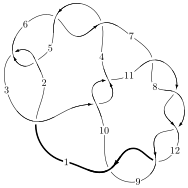
\includegraphics[width=112pt]{../../../GIT/diagram.site/Diagrams/png/1223_12a_0422.png}\\
\ \ \ A knot diagram\footnotemark}&
\allowdisplaybreaks
\textbf{Linearized knot diagam} \\
\cline{2-2}
 &
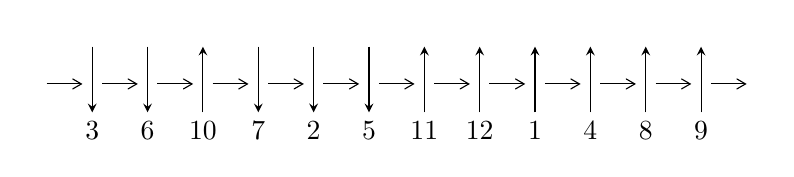
\begin{tikzpicture}[x=20pt, y=17pt]
	% nodes
	\node (C0) at (0, 0) {};
	\node (C1) at (1, 0) {};
	\node (C1U) at (1, +1) {};
	\node (C1D) at (1, -1) {3};

	\node (C2) at (2, 0) {};
	\node (C2U) at (2, +1) {};
	\node (C2D) at (2, -1) {6};

	\node (C3) at (3, 0) {};
	\node (C3U) at (3, +1) {};
	\node (C3D) at (3, -1) {10};

	\node (C4) at (4, 0) {};
	\node (C4U) at (4, +1) {};
	\node (C4D) at (4, -1) {7};

	\node (C5) at (5, 0) {};
	\node (C5U) at (5, +1) {};
	\node (C5D) at (5, -1) {2};

	\node (C6) at (6, 0) {};
	\node (C6U) at (6, +1) {};
	\node (C6D) at (6, -1) {5};

	\node (C7) at (7, 0) {};
	\node (C7U) at (7, +1) {};
	\node (C7D) at (7, -1) {11};

	\node (C8) at (8, 0) {};
	\node (C8U) at (8, +1) {};
	\node (C8D) at (8, -1) {12};

	\node (C9) at (9, 0) {};
	\node (C9U) at (9, +1) {};
	\node (C9D) at (9, -1) {1};

	\node (C10) at (10, 0) {};
	\node (C10U) at (10, +1) {};
	\node (C10D) at (10, -1) {4};

	\node (C11) at (11, 0) {};
	\node (C11U) at (11, +1) {};
	\node (C11D) at (11, -1) {8};

	\node (C12) at (12, 0) {};
	\node (C12U) at (12, +1) {};
	\node (C12D) at (12, -1) {9};
	\node (C13) at (13, 0) {};

	% arrows
	\draw[->,>={angle 60}]
	(C0) edge (C1) (C1) edge (C2) (C2) edge (C3) (C3) edge (C4) (C4) edge (C5) (C5) edge (C6) (C6) edge (C7) (C7) edge (C8) (C8) edge (C9) (C9) edge (C10) (C10) edge (C11) (C11) edge (C12) (C12) edge (C13) ;	\draw[->,>=stealth]
	(C1U) edge (C1D) (C2U) edge (C2D) (C3D) edge (C3U) (C4U) edge (C4D) (C5U) edge (C5D) (C6U) edge (C6D) (C7D) edge (C7U) (C8D) edge (C8U) (C9D) edge (C9U) (C10D) edge (C10U) (C11D) edge (C11U) (C12D) edge (C12U) ;
	\end{tikzpicture} \\
\hhline{~~} \\& 
\textbf{Solving Sequence} \\ \cline{2-2} 
 &
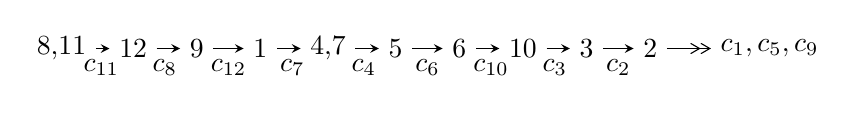
\begin{tikzpicture}[x=23pt, y=7pt]
	% node
	\node (A0) at (-1/8, 0) {8,11};
	\node (A1) at (1, 0) {12};
	\node (A2) at (2, 0) {9};
	\node (A3) at (3, 0) {1};
	\node (A4) at (65/16, 0) {4,7};
	\node (A5) at (41/8, 0) {5};
	\node (A6) at (49/8, 0) {6};
	\node (A7) at (57/8, 0) {10};
	\node (A8) at (65/8, 0) {3};
	\node (A9) at (73/8, 0) {2};
	\node (C1) at (1/2, -1) {$c_{11}$};
	\node (C2) at (3/2, -1) {$c_{8}$};
	\node (C3) at (5/2, -1) {$c_{12}$};
	\node (C4) at (7/2, -1) {$c_{7}$};
	\node (C5) at (37/8, -1) {$c_{4}$};
	\node (C6) at (45/8, -1) {$c_{6}$};
	\node (C7) at (53/8, -1) {$c_{10}$};
	\node (C8) at (61/8, -1) {$c_{3}$};
	\node (C9) at (69/8, -1) {$c_{2}$};
	\node (A10) at (11, 0) {$c_{1},c_{5},c_{9}$};

	% edge
	\draw[->,>=stealth]	
	(A0) edge (A1) (A1) edge (A2) (A2) edge (A3) (A3) edge (A4) (A4) edge (A5) (A5) edge (A6) (A6) edge (A7) (A7) edge (A8) (A8) edge (A9) ;
	\draw[->>,>={angle 60}]	
	(A9) edge (A10);
\end{tikzpicture} \\ 

\end{tabular} \\

\footnotetext{
The image of knot diagram is generated by the software ``\textbf{Draw programme}" developed by Andrew Bartholomew(\url{http://www.layer8.co.uk/maths/draw/index.htm\#Running-draw}), where we modified some parts for our purpose(\url{https://github.com/CATsTAILs/LinksPainter}).
}\phantom \\ \newline 
\centering \textbf{Ideals for irreducible components\footnotemark of $X_{\text{par}}$} 
 
\begin{align*}
I^u_{1}&=\langle 
-47 u^{38}+152 u^{37}+\cdots+2 b+26,\;101 u^{38}-320 u^{37}+\cdots+4 a-62,\;u^{39}-5 u^{38}+\cdots- u+1\rangle \\
I^u_{2}&=\langle 
b,\;a^3- a^2 u- a^2+2 a u+4 a-2 u-3,\;u^2+u-1\rangle \\
I^u_{3}&=\langle 
b+1,\;a-2,\;u+1\rangle \\
\\
\end{align*}
\raggedright * 3 irreducible components of $\dim_{\mathbb{C}}=0$, with total 46 representations.\\
\footnotetext{All coefficients of polynomials are rational numbers. But the coefficients are sometimes approximated in decimal forms when there is not enough margin.}
\newpage
\renewcommand{\arraystretch}{1}
\centering \section*{I. $I^u_{1}= \langle -47 u^{38}+152 u^{37}+\cdots+2 b+26,\;101 u^{38}-320 u^{37}+\cdots+4 a-62,\;u^{39}-5 u^{38}+\cdots- u+1 \rangle$}
\flushleft \textbf{(i) Arc colorings}\\
\begin{tabular}{m{7pt} m{180pt} m{7pt} m{180pt} }
\flushright $a_{8}=$&$\begin{pmatrix}0\\u\end{pmatrix}$ \\
\flushright $a_{11}=$&$\begin{pmatrix}1\\0\end{pmatrix}$ \\
\flushright $a_{12}=$&$\begin{pmatrix}1\\- u^2\end{pmatrix}$ \\
\flushright $a_{9}=$&$\begin{pmatrix}u\\- u^3+u\end{pmatrix}$ \\
\flushright $a_{1}=$&$\begin{pmatrix}- u^2+1\\u^4-2 u^2\end{pmatrix}$ \\
\flushright $a_{4}=$&$\begin{pmatrix}-\frac{101}{4} u^{38}+80 u^{37}+\cdots-\frac{27}{4} u+\frac{31}{2}\\\frac{47}{2} u^{38}-76 u^{37}+\cdots+\frac{11}{2} u-13\end{pmatrix}$ \\
\flushright $a_{7}=$&$\begin{pmatrix}- u\\u\end{pmatrix}$ \\
\flushright $a_{5}=$&$\begin{pmatrix}-17.2500 u^{38}+54.7500 u^{37}+\cdots-3.75000 u+10.7500\\\frac{31}{2} u^{38}-\frac{203}{4} u^{37}+\cdots+\frac{5}{2} u-\frac{33}{4}\end{pmatrix}$ \\
\flushright $a_{6}=$&$\begin{pmatrix}-\frac{1}{2} u^{38}+\frac{7}{4} u^{37}+\cdots-6 u+\frac{5}{4}\\\frac{3}{4} u^{38}-\frac{5}{2} u^{37}+\cdots+\frac{1}{4} u-\frac{1}{2}\end{pmatrix}$ \\
\flushright $a_{10}=$&$\begin{pmatrix}- u^3+2 u\\u^5-3 u^3+u\end{pmatrix}$ \\
\flushright $a_{3}=$&$\begin{pmatrix}\frac{93}{4} u^{38}-77 u^{37}+\cdots+\frac{19}{4} u-\frac{23}{2}\\-\frac{75}{2} u^{38}+122 u^{37}+\cdots-\frac{19}{2} u+22\end{pmatrix}$ \\
\flushright $a_{2}=$&$\begin{pmatrix}-\frac{1}{4} u^{38}+\frac{3}{4} u^{37}+\cdots+\frac{19}{4} u+\frac{1}{4}\\u^{11}-7 u^9+16 u^7-2 u^6-13 u^5+8 u^4+3 u^3-6 u^2+u\end{pmatrix}$\\&\end{tabular}
\flushleft \textbf{(ii) Obstruction class $= -1$}\\~\\
\flushleft \textbf{(iii) Cusp Shapes $= -64 u^{38}+210 u^{37}+\cdots-6 u+\frac{81}{2}$}\\~\\
\newpage\renewcommand{\arraystretch}{1}
\flushleft \textbf{(iv) u-Polynomials at the component}\newline \\
\begin{tabular}{m{50pt}|m{274pt}}
Crossings & \hspace{64pt}u-Polynomials at each crossing \\
\hline $$\begin{aligned}c_{1},c_{4},c_{6}\end{aligned}$$&$\begin{aligned}
&u^{39}+8 u^{38}+\cdots+42 u+1
\end{aligned}$\\
\hline $$\begin{aligned}c_{2},c_{5}\end{aligned}$$&$\begin{aligned}
&u^{39}+2 u^{38}+\cdots-6 u+1
\end{aligned}$\\
\hline $$\begin{aligned}c_{3},c_{10}\end{aligned}$$&$\begin{aligned}
&u^{39}+2 u^{38}+\cdots-160 u-64
\end{aligned}$\\
\hline $$\begin{aligned}c_{7},c_{8},c_{9}\\c_{11},c_{12}\end{aligned}$$&$\begin{aligned}
&u^{39}-5 u^{38}+\cdots- u+1
\end{aligned}$\\
\hline
\end{tabular}\\~\\
\newpage\renewcommand{\arraystretch}{1}
\flushleft \textbf{(v) Riley Polynomials at the component}\newline \\
\begin{tabular}{m{50pt}|m{274pt}}
Crossings & \hspace{64pt}Riley Polynomials at each crossing \\
\hline $$\begin{aligned}c_{1},c_{4},c_{6}\end{aligned}$$&$\begin{aligned}
&y^{39}+48 y^{38}+\cdots+978 y-1
\end{aligned}$\\
\hline $$\begin{aligned}c_{2},c_{5}\end{aligned}$$&$\begin{aligned}
&y^{39}-8 y^{38}+\cdots+42 y-1
\end{aligned}$\\
\hline $$\begin{aligned}c_{3},c_{10}\end{aligned}$$&$\begin{aligned}
&y^{39}-34 y^{38}+\cdots+25600 y-4096
\end{aligned}$\\
\hline $$\begin{aligned}c_{7},c_{8},c_{9}\\c_{11},c_{12}\end{aligned}$$&$\begin{aligned}
&y^{39}-55 y^{38}+\cdots-9 y-1
\end{aligned}$\\
\hline
\end{tabular}\\~\\
\newpage\flushleft \textbf{(vi) Complex Volumes and Cusp Shapes}
$$\begin{array}{c|c|c}  
\text{Solutions to }I^u_{1}& \I (\text{vol} + \sqrt{-1}CS) & \text{Cusp shape}\\
 \hline 
\begin{aligned}
u &= -1.053960 + 0.224778 I \\
a &= \phantom{-}1.61876 + 0.68220 I \\
b &= -1.163720 + 0.312418 I\end{aligned}
 & \phantom{-}4.49453 - 5.61479 I & \phantom{-}8.25857 + 7.26249 I \\ \hline\begin{aligned}
u &= -1.053960 - 0.224778 I \\
a &= \phantom{-}1.61876 - 0.68220 I \\
b &= -1.163720 - 0.312418 I\end{aligned}
 & \phantom{-}4.49453 + 5.61479 I & \phantom{-}8.25857 - 7.26249 I \\ \hline\begin{aligned}
u &= \phantom{-}0.862747 + 0.116296 I \\
a &= -0.069535 - 0.131159 I \\
b &= -0.221452 + 0.784770 I\end{aligned}
 & \phantom{-}1.42290 + 1.53553 I & \phantom{-}7.01176 - 4.72842 I \\ \hline\begin{aligned}
u &= \phantom{-}0.862747 - 0.116296 I \\
a &= -0.069535 + 0.131159 I \\
b &= -0.221452 - 0.784770 I\end{aligned}
 & \phantom{-}1.42290 - 1.53553 I & \phantom{-}7.01176 + 4.72842 I \\ \hline\begin{aligned}
u &= \phantom{-}1.139060 + 0.026381 I \\
a &= -0.038812 + 0.168804 I \\
b &= -0.025448 + 1.175110 I\end{aligned}
 & \phantom{-}8.36476 + 3.13639 I & \phantom{-0.000000 } 0 \\ \hline\begin{aligned}
u &= \phantom{-}1.139060 - 0.026381 I \\
a &= -0.038812 - 0.168804 I \\
b &= -0.025448 - 1.175110 I\end{aligned}
 & \phantom{-}8.36476 - 3.13639 I & \phantom{-0.000000 } 0 \\ \hline\begin{aligned}
u &= -1.151060 + 0.133458 I \\
a &= -1.46113 - 0.36382 I \\
b &= \phantom{-}1.226750 - 0.126705 I\end{aligned}
 & \phantom{-}6.34383 - 1.26782 I & \phantom{-0.000000 } 0 \\ \hline\begin{aligned}
u &= -1.151060 - 0.133458 I \\
a &= -1.46113 + 0.36382 I \\
b &= \phantom{-}1.226750 + 0.126705 I\end{aligned}
 & \phantom{-}6.34383 + 1.26782 I & \phantom{-0.000000 } 0 \\ \hline\begin{aligned}
u &= \phantom{-}0.415029 + 0.681141 I \\
a &= -0.293962 - 0.902195 I \\
b &= -1.43879 - 0.09612 I\end{aligned}
 & \phantom{-}8.68168 - 1.01341 I & \phantom{-}8.20452 - 0.45089 I \\ \hline\begin{aligned}
u &= \phantom{-}0.415029 - 0.681141 I \\
a &= -0.293962 + 0.902195 I \\
b &= -1.43879 + 0.09612 I\end{aligned}
 & \phantom{-}8.68168 + 1.01341 I & \phantom{-}8.20452 + 0.45089 I\\
 \hline 
 \end{array}$$\newpage$$\begin{array}{c|c|c}  
\text{Solutions to }I^u_{1}& \I (\text{vol} + \sqrt{-1}CS) & \text{Cusp shape}\\
 \hline 
\begin{aligned}
u &= \phantom{-}0.379187 + 0.691000 I \\
a &= \phantom{-}0.296338 + 0.946075 I \\
b &= \phantom{-}1.43542 + 0.18852 I\end{aligned}
 & \phantom{-}8.57368 + 5.46017 I & \phantom{-}7.82438 - 5.30651 I \\ \hline\begin{aligned}
u &= \phantom{-}0.379187 - 0.691000 I \\
a &= \phantom{-}0.296338 - 0.946075 I \\
b &= \phantom{-}1.43542 - 0.18852 I\end{aligned}
 & \phantom{-}8.57368 - 5.46017 I & \phantom{-}7.82438 + 5.30651 I \\ \hline\begin{aligned}
u &= -1.160140 + 0.396351 I \\
a &= \phantom{-}1.23807 + 0.87778 I \\
b &= -1.52336 + 0.47798 I\end{aligned}
 & \phantom{-}13.3910 - 9.1863 I & \phantom{-0.000000 } 0 \\ \hline\begin{aligned}
u &= -1.160140 - 0.396351 I \\
a &= \phantom{-}1.23807 - 0.87778 I \\
b &= -1.52336 - 0.47798 I\end{aligned}
 & \phantom{-}13.3910 + 9.1863 I & \phantom{-0.000000 } 0 \\ \hline\begin{aligned}
u &= -1.187780 + 0.377695 I \\
a &= -1.21277 - 0.82919 I \\
b &= \phantom{-}1.54397 - 0.40480 I\end{aligned}
 & \phantom{-}13.72490 - 2.63237 I & \phantom{-0.000000 } 0 \\ \hline\begin{aligned}
u &= -1.187780 - 0.377695 I \\
a &= -1.21277 + 0.82919 I \\
b &= \phantom{-}1.54397 + 0.40480 I\end{aligned}
 & \phantom{-}13.72490 + 2.63237 I & \phantom{-0.000000 } 0 \\ \hline\begin{aligned}
u &= \phantom{-}0.467926 + 0.375228 I \\
a &= \phantom{-}0.068401 - 0.656383 I \\
b &= -0.834315 + 0.134239 I\end{aligned}
 & \phantom{-}1.190300 - 0.320599 I & \phantom{-}8.01474 - 0.06231 I \\ \hline\begin{aligned}
u &= \phantom{-}0.467926 - 0.375228 I \\
a &= \phantom{-}0.068401 + 0.656383 I \\
b &= -0.834315 - 0.134239 I\end{aligned}
 & \phantom{-}1.190300 + 0.320599 I & \phantom{-}8.01474 + 0.06231 I \\ \hline\begin{aligned}
u &= \phantom{-}0.239901 + 0.477819 I \\
a &= -0.049714 + 1.108090 I \\
b &= \phantom{-}0.899573 + 0.293268 I\end{aligned}
 & \phantom{-}0.46281 + 3.25190 I & \phantom{-}3.30026 - 8.26387 I \\ \hline\begin{aligned}
u &= \phantom{-}0.239901 - 0.477819 I \\
a &= -0.049714 - 1.108090 I \\
b &= \phantom{-}0.899573 - 0.293268 I\end{aligned}
 & \phantom{-}0.46281 - 3.25190 I & \phantom{-}3.30026 + 8.26387 I\\
 \hline 
 \end{array}$$\newpage$$\begin{array}{c|c|c}  
\text{Solutions to }I^u_{1}& \I (\text{vol} + \sqrt{-1}CS) & \text{Cusp shape}\\
 \hline 
\begin{aligned}
u &= \phantom{-}0.487731\phantom{ +0.000000I} \\
a &= \phantom{-}0.343685\phantom{ +0.000000I} \\
b &= -0.408979\phantom{ +0.000000I}\end{aligned}
 & \phantom{-}0.740705\phantom{ +0.000000I} & \phantom{-}13.6330\phantom{ +0.000000I} \\ \hline\begin{aligned}
u &= -1.59861\phantom{ +0.000000I} \\
a &= -0.240120\phantom{ +0.000000I} \\
b &= \phantom{-}0.465924\phantom{ +0.000000I}\end{aligned}
 & \phantom{-}8.08529\phantom{ +0.000000I} & \phantom{-0.000000 } 0 \\ \hline\begin{aligned}
u &= -0.345833 + 0.036532 I \\
a &= \phantom{-}0.12571 + 3.44175 I \\
b &= -0.000094 + 0.479895 I\end{aligned}
 & \phantom{-}3.55637 - 2.89653 I & -3.84297 + 3.88300 I \\ \hline\begin{aligned}
u &= -0.345833 - 0.036532 I \\
a &= \phantom{-}0.12571 - 3.44175 I \\
b &= -0.000094 - 0.479895 I\end{aligned}
 & \phantom{-}3.55637 + 2.89653 I & -3.84297 - 3.88300 I \\ \hline\begin{aligned}
u &= -1.67511 + 0.02701 I \\
a &= -0.088705 - 0.412032 I \\
b &= \phantom{-}0.229021 + 0.890141 I\end{aligned}
 & \phantom{-}10.40850 - 2.06539 I & \phantom{-0.000000 } 0 \\ \hline\begin{aligned}
u &= -1.67511 - 0.02701 I \\
a &= -0.088705 + 0.412032 I \\
b &= \phantom{-}0.229021 - 0.890141 I\end{aligned}
 & \phantom{-}10.40850 + 2.06539 I & \phantom{-0.000000 } 0 \\ \hline\begin{aligned}
u &= \phantom{-}1.73748\phantom{ +0.000000I} \\
a &= -2.04429\phantom{ +0.000000I} \\
b &= \phantom{-}1.35510\phantom{ +0.000000I}\end{aligned}
 & \phantom{-}11.5719\phantom{ +0.000000I} & \phantom{-0.000000 } 0 \\ \hline\begin{aligned}
u &= \phantom{-}1.74621 + 0.05370 I \\
a &= -1.91054 + 0.23326 I \\
b &= \phantom{-}1.42871 + 0.37526 I\end{aligned}
 & \phantom{-}14.5888 + 6.7421 I & \phantom{-0.000000 } 0 \\ \hline\begin{aligned}
u &= \phantom{-}1.74621 - 0.05370 I \\
a &= -1.91054 - 0.23326 I \\
b &= \phantom{-}1.42871 - 0.37526 I\end{aligned}
 & \phantom{-}14.5888 - 6.7421 I & \phantom{-0.000000 } 0 \\ \hline\begin{aligned}
u &= -1.76716 + 0.00715 I \\
a &= -0.013757 - 0.629655 I \\
b &= \phantom{-}0.04950 + 1.56385 I\end{aligned}
 & \phantom{-}18.9593 - 3.2843 I & \phantom{-0.000000 } 0\\
 \hline 
 \end{array}$$\newpage$$\begin{array}{c|c|c}  
\text{Solutions to }I^u_{1}& \I (\text{vol} + \sqrt{-1}CS) & \text{Cusp shape}\\
 \hline 
\begin{aligned}
u &= -1.76716 - 0.00715 I \\
a &= -0.013757 + 0.629655 I \\
b &= \phantom{-}0.04950 - 1.56385 I\end{aligned}
 & \phantom{-}18.9593 + 3.2843 I & \phantom{-0.000000 } 0 \\ \hline\begin{aligned}
u &= \phantom{-}1.76755 + 0.03169 I \\
a &= \phantom{-}1.88452 - 0.11380 I \\
b &= -1.56905 - 0.21871 I\end{aligned}
 & \phantom{-}16.9501 + 1.9651 I & \phantom{-0.000000 } 0 \\ \hline\begin{aligned}
u &= \phantom{-}1.76755 - 0.03169 I \\
a &= \phantom{-}1.88452 + 0.11380 I \\
b &= -1.56905 + 0.21871 I\end{aligned}
 & \phantom{-}16.9501 - 1.9651 I & \phantom{-0.000000 } 0 \\ \hline\begin{aligned}
u &= \phantom{-}1.77210 + 0.10705 I \\
a &= -1.71021 + 0.26961 I \\
b &= \phantom{-}1.61742 + 0.71877 I\end{aligned}
 & -15.5908 + 11.3747 I & \phantom{-0.000000 } 0 \\ \hline\begin{aligned}
u &= \phantom{-}1.77210 - 0.10705 I \\
a &= -1.71021 - 0.26961 I \\
b &= \phantom{-}1.61742 - 0.71877 I\end{aligned}
 & -15.5908 - 11.3747 I & \phantom{-0.000000 } 0 \\ \hline\begin{aligned}
u &= -0.042751 + 0.219509 I \\
a &= -0.63189 + 2.24770 I \\
b &= \phantom{-}0.311409 + 0.398108 I\end{aligned}
 & -1.261040 - 0.319837 I & -6.08687 + 0.82925 I \\ \hline\begin{aligned}
u &= -0.042751 - 0.219509 I \\
a &= -0.63189 - 2.24770 I \\
b &= \phantom{-}0.311409 - 0.398108 I\end{aligned}
 & -1.261040 + 0.319837 I & -6.08687 - 0.82925 I \\ \hline\begin{aligned}
u &= \phantom{-}1.78078 + 0.09884 I \\
a &= \phantom{-}1.71959 - 0.23944 I \\
b &= -1.67156 - 0.66408 I\end{aligned}
 & -15.0724 + 4.7212 I & \phantom{-0.000000 } 0 \\ \hline\begin{aligned}
u &= \phantom{-}1.78078 - 0.09884 I \\
a &= \phantom{-}1.71959 + 0.23944 I \\
b &= -1.67156 + 0.66408 I\end{aligned}
 & -15.0724 - 4.7212 I & \phantom{-0.000000 } 0\\
 \hline 
 \end{array}$$\newpage\newpage\renewcommand{\arraystretch}{1}
\centering \section*{II. $I^u_{2}= \langle b,\;a^3- a^2 u- a^2+2 a u+4 a-2 u-3,\;u^2+u-1 \rangle$}
\flushleft \textbf{(i) Arc colorings}\\
\begin{tabular}{m{7pt} m{180pt} m{7pt} m{180pt} }
\flushright $a_{8}=$&$\begin{pmatrix}0\\u\end{pmatrix}$ \\
\flushright $a_{11}=$&$\begin{pmatrix}1\\0\end{pmatrix}$ \\
\flushright $a_{12}=$&$\begin{pmatrix}1\\u-1\end{pmatrix}$ \\
\flushright $a_{9}=$&$\begin{pmatrix}u\\- u+1\end{pmatrix}$ \\
\flushright $a_{1}=$&$\begin{pmatrix}u\\- u\end{pmatrix}$ \\
\flushright $a_{4}=$&$\begin{pmatrix}a\\0\end{pmatrix}$ \\
\flushright $a_{7}=$&$\begin{pmatrix}- u\\u\end{pmatrix}$ \\
\flushright $a_{5}=$&$\begin{pmatrix}a u\\- a u+a\end{pmatrix}$ \\
\flushright $a_{6}=$&$\begin{pmatrix}- a^2 u+a^2- u\\2 a^2 u- a^2+u\end{pmatrix}$ \\
\flushright $a_{10}=$&$\begin{pmatrix}1\\0\end{pmatrix}$ \\
\flushright $a_{3}=$&$\begin{pmatrix}a\\0\end{pmatrix}$ \\
\flushright $a_{2}=$&$\begin{pmatrix}a^2 u+u\\- u\end{pmatrix}$\\&\end{tabular}
\flushleft \textbf{(ii) Obstruction class $= 1$}\\~\\
\flushleft \textbf{(iii) Cusp Shapes $= 10 a^2 u-9 a^2+6 a u- a+3 u-1$}\\~\\
\newpage\renewcommand{\arraystretch}{1}
\flushleft \textbf{(iv) u-Polynomials at the component}\newline \\
\begin{tabular}{m{50pt}|m{274pt}}
Crossings & \hspace{64pt}u-Polynomials at each crossing \\
\hline $$\begin{aligned}c_{1},c_{4}\end{aligned}$$&$\begin{aligned}
&(u^3- u^2+2 u-1)^2
\end{aligned}$\\
\hline $$\begin{aligned}c_{2}\end{aligned}$$&$\begin{aligned}
&(u^3+u^2-1)^2
\end{aligned}$\\
\hline $$\begin{aligned}c_{3},c_{10}\end{aligned}$$&$\begin{aligned}
&u^6
\end{aligned}$\\
\hline $$\begin{aligned}c_{5}\end{aligned}$$&$\begin{aligned}
&(u^3- u^2+1)^2
\end{aligned}$\\
\hline $$\begin{aligned}c_{6}\end{aligned}$$&$\begin{aligned}
&(u^3+u^2+2 u+1)^2
\end{aligned}$\\
\hline $$\begin{aligned}c_{7},c_{8},c_{9}\end{aligned}$$&$\begin{aligned}
&(u^2- u-1)^3
\end{aligned}$\\
\hline $$\begin{aligned}c_{11},c_{12}\end{aligned}$$&$\begin{aligned}
&(u^2+u-1)^3
\end{aligned}$\\
\hline
\end{tabular}\\~\\
\newpage\renewcommand{\arraystretch}{1}
\flushleft \textbf{(v) Riley Polynomials at the component}\newline \\
\begin{tabular}{m{50pt}|m{274pt}}
Crossings & \hspace{64pt}Riley Polynomials at each crossing \\
\hline $$\begin{aligned}c_{1},c_{4},c_{6}\end{aligned}$$&$\begin{aligned}
&(y^3+3 y^2+2 y-1)^2
\end{aligned}$\\
\hline $$\begin{aligned}c_{2},c_{5}\end{aligned}$$&$\begin{aligned}
&(y^3- y^2+2 y-1)^2
\end{aligned}$\\
\hline $$\begin{aligned}c_{3},c_{10}\end{aligned}$$&$\begin{aligned}
&y^6
\end{aligned}$\\
\hline $$\begin{aligned}c_{7},c_{8},c_{9}\\c_{11},c_{12}\end{aligned}$$&$\begin{aligned}
&(y^2-3 y+1)^3
\end{aligned}$\\
\hline
\end{tabular}\\~\\
\newpage\flushleft \textbf{(vi) Complex Volumes and Cusp Shapes}
$$\begin{array}{c|c|c}  
\text{Solutions to }I^u_{2}& \I (\text{vol} + \sqrt{-1}CS) & \text{Cusp shape}\\
 \hline 
\begin{aligned}
u &= \phantom{-}0.618034\phantom{ +0.000000I} \\
a &= \phantom{-}0.922021\phantom{ +0.000000I} \\
b &= \phantom{-0.000000 } 0\end{aligned}
 & -0.126494\phantom{ +0.000000I} & \phantom{-}0.954070\phantom{ +0.000000I} \\ \hline\begin{aligned}
u &= \phantom{-}0.618034\phantom{ +0.000000I} \\
a &= \phantom{-}0.34801 + 2.11500 I \\
b &= \phantom{-0.000000 } 0\end{aligned}
 & \phantom{-}4.01109 - 2.82812 I & \phantom{-}14.0681 + 1.5771 I \\ \hline\begin{aligned}
u &= \phantom{-}0.618034\phantom{ +0.000000I} \\
a &= \phantom{-}0.34801 - 2.11500 I \\
b &= \phantom{-0.000000 } 0\end{aligned}
 & \phantom{-}4.01109 + 2.82812 I & \phantom{-}14.0681 - 1.5771 I \\ \hline\begin{aligned}
u &= -1.61803\phantom{ +0.000000I} \\
a &= -0.132927 + 0.807858 I \\
b &= \phantom{-0.000000 } 0\end{aligned}
 & \phantom{-}11.90680 + 2.82812 I & \phantom{-}11.55793 - 3.24268 I \\ \hline\begin{aligned}
u &= -1.61803\phantom{ +0.000000I} \\
a &= -0.132927 - 0.807858 I \\
b &= \phantom{-0.000000 } 0\end{aligned}
 & \phantom{-}11.90680 - 2.82812 I & \phantom{-}11.55793 + 3.24268 I \\ \hline\begin{aligned}
u &= -1.61803\phantom{ +0.000000I} \\
a &= -0.352181\phantom{ +0.000000I} \\
b &= \phantom{-0.000000 } 0\end{aligned}
 & \phantom{-}7.76919\phantom{ +0.000000I} & -5.20600\phantom{ +0.000000I}\\
 \hline 
 \end{array}$$\newpage\newpage\renewcommand{\arraystretch}{1}
\centering \section*{III. $I^u_{3}= \langle b+1,\;a-2,\;u+1 \rangle$}
\flushleft \textbf{(i) Arc colorings}\\
\begin{tabular}{m{7pt} m{180pt} m{7pt} m{180pt} }
\flushright $a_{8}=$&$\begin{pmatrix}0\\-1\end{pmatrix}$ \\
\flushright $a_{11}=$&$\begin{pmatrix}1\\0\end{pmatrix}$ \\
\flushright $a_{12}=$&$\begin{pmatrix}1\\-1\end{pmatrix}$ \\
\flushright $a_{9}=$&$\begin{pmatrix}-1\\0\end{pmatrix}$ \\
\flushright $a_{1}=$&$\begin{pmatrix}0\\-1\end{pmatrix}$ \\
\flushright $a_{4}=$&$\begin{pmatrix}2\\-1\end{pmatrix}$ \\
\flushright $a_{7}=$&$\begin{pmatrix}1\\-1\end{pmatrix}$ \\
\flushright $a_{5}=$&$\begin{pmatrix}1\\0\end{pmatrix}$ \\
\flushright $a_{6}=$&$\begin{pmatrix}0\\-1\end{pmatrix}$ \\
\flushright $a_{10}=$&$\begin{pmatrix}-1\\1\end{pmatrix}$ \\
\flushright $a_{3}=$&$\begin{pmatrix}1\\0\end{pmatrix}$ \\
\flushright $a_{2}=$&$\begin{pmatrix}1\\-1\end{pmatrix}$\\&\end{tabular}
\flushleft \textbf{(ii) Obstruction class $= -1$}\\~\\
\flushleft \textbf{(iii) Cusp Shapes $= 6$}\\~\\
\newpage\renewcommand{\arraystretch}{1}
\flushleft \textbf{(iv) u-Polynomials at the component}\newline \\
\begin{tabular}{m{50pt}|m{274pt}}
Crossings & \hspace{64pt}u-Polynomials at each crossing \\
\hline $$\begin{aligned}c_{1},c_{2},c_{4}\\c_{5},c_{6},c_{7}\\c_{8},c_{9},c_{11}\\c_{12}\end{aligned}$$&$\begin{aligned}
&u+1
\end{aligned}$\\
\hline $$\begin{aligned}c_{3},c_{10}\end{aligned}$$&$\begin{aligned}
&u-1
\end{aligned}$\\
\hline
\end{tabular}\\~\\
\newpage\renewcommand{\arraystretch}{1}
\flushleft \textbf{(v) Riley Polynomials at the component}\newline \\
\begin{tabular}{m{50pt}|m{274pt}}
Crossings & \hspace{64pt}Riley Polynomials at each crossing \\
\hline $$\begin{aligned}c_{1},c_{2},c_{3}\\c_{4},c_{5},c_{6}\\c_{7},c_{8},c_{9}\\c_{10},c_{11},c_{12}\end{aligned}$$&$\begin{aligned}
&y-1
\end{aligned}$\\
\hline
\end{tabular}\\~\\
\newpage\flushleft \textbf{(vi) Complex Volumes and Cusp Shapes}
$$\begin{array}{c|c|c}  
\text{Solutions to }I^u_{3}& \I (\text{vol} + \sqrt{-1}CS) & \text{Cusp shape}\\
 \hline 
\begin{aligned}
u &= -1.00000\phantom{ +0.000000I} \\
a &= \phantom{-}2.00000\phantom{ +0.000000I} \\
b &= -1.00000\phantom{ +0.000000I}\end{aligned}
 & \phantom{-}1.64493\phantom{ +0.000000I} & \phantom{-}6.00000\phantom{ +0.000000I}\\
 \hline 
 \end{array}$$\newpage
\newpage\renewcommand{\arraystretch}{1}
\centering \section*{ IV. u-Polynomials}
\begin{tabular}{m{50pt}|m{274pt}}
Crossings & \hspace{64pt}u-Polynomials at each crossing \\
\hline $$\begin{aligned}c_{1},c_{4}\end{aligned}$$&$\begin{aligned}
&(u+1)(u^3- u^2+2 u-1)^2(u^{39}+8 u^{38}+\cdots+42 u+1)
\end{aligned}$\\
\hline $$\begin{aligned}c_{2}\end{aligned}$$&$\begin{aligned}
&(u+1)(u^3+u^2-1)^2(u^{39}+2 u^{38}+\cdots-6 u+1)
\end{aligned}$\\
\hline $$\begin{aligned}c_{3},c_{10}\end{aligned}$$&$\begin{aligned}
&u^6(u-1)(u^{39}+2 u^{38}+\cdots-160 u-64)
\end{aligned}$\\
\hline $$\begin{aligned}c_{5}\end{aligned}$$&$\begin{aligned}
&(u+1)(u^3- u^2+1)^2(u^{39}+2 u^{38}+\cdots-6 u+1)
\end{aligned}$\\
\hline $$\begin{aligned}c_{6}\end{aligned}$$&$\begin{aligned}
&(u+1)(u^3+u^2+2 u+1)^2(u^{39}+8 u^{38}+\cdots+42 u+1)
\end{aligned}$\\
\hline $$\begin{aligned}c_{7},c_{8},c_{9}\end{aligned}$$&$\begin{aligned}
&(u+1)(u^2- u-1)^3(u^{39}-5 u^{38}+\cdots- u+1)
\end{aligned}$\\
\hline $$\begin{aligned}c_{11},c_{12}\end{aligned}$$&$\begin{aligned}
&(u+1)(u^2+u-1)^3(u^{39}-5 u^{38}+\cdots- u+1)
\end{aligned}$\\
\hline
\end{tabular}\newpage\renewcommand{\arraystretch}{1}
\centering \section*{ V. Riley Polynomials}
\begin{tabular}{m{50pt}|m{274pt}}
Crossings & \hspace{64pt}Riley Polynomials at each crossing \\
\hline $$\begin{aligned}c_{1},c_{4},c_{6}\end{aligned}$$&$\begin{aligned}
&(y-1)(y^3+3 y^2+2 y-1)^2(y^{39}+48 y^{38}+\cdots+978 y-1)
\end{aligned}$\\
\hline $$\begin{aligned}c_{2},c_{5}\end{aligned}$$&$\begin{aligned}
&(y-1)(y^3- y^2+2 y-1)^2(y^{39}-8 y^{38}+\cdots+42 y-1)
\end{aligned}$\\
\hline $$\begin{aligned}c_{3},c_{10}\end{aligned}$$&$\begin{aligned}
&y^6(y-1)(y^{39}-34 y^{38}+\cdots+25600 y-4096)
\end{aligned}$\\
\hline $$\begin{aligned}c_{7},c_{8},c_{9}\\c_{11},c_{12}\end{aligned}$$&$\begin{aligned}
&(y-1)(y^2-3 y+1)^3(y^{39}-55 y^{38}+\cdots-9 y-1)
\end{aligned}$\\
\hline
\end{tabular}
\vskip 2pc
\end{document}